% Paquets généraux
\documentclass[a4paper,12pt,titlepage]{article}
\usepackage[T1]{fontenc}
\usepackage[utf8]{inputenc}
\usepackage[french]{babel}
\usepackage[gen]{eurosym}
%\usepackage[dvips]{graphicx}
\usepackage{fancyhdr}
\usepackage{pdfpages} 
\usepackage{multido}
\usepackage{hyperref}
%\usepackage{textcomp}
%\usepackage{aeguill}
\usepackage{schemabloc}
\usepackage[bitstream-charter]{mathdesign}

\newcommand{\id}{54}
\newcommand{\nom}{Liaisons mécaniques}
\newcommand{\sequence}{04}
\newcommand{\num}{01}
\newcommand{\type}{TP}
\newcommand{\descrip}{Modélisation d'un solide. Comportement des liaisons mécaniques. Modéliser les mécanismes du laboratoire par un schéma cinématique, paramétré.}
\newcommand{\competences}{A3-C4: Analyse d'architecture et de comportement \\ &  Mod1-C1: Isolement d'un solide ou d'un système de solides \\ &  Mod2-C10-1: Modèle de solide indéformable \\ &  Mod2-C11: Modélisation géométrique et cinématique des mouvements entre solides indéformables \\ &  Mod2-C12: Modélisation cinématique des liaisons entre solides \\ &  Mod2-C15: Modélisation des actions mécaniques \\ &  Rés-C6: Utilisation d'un solveur ou d'un logiciel multi physique \\ &  Com1-C1: Différents descripteurs introduits dans le programme \\ &  Com2-C4: Outils de communication}
\newcommand{\nbcomp}{9}
\newcommand{\systemes}{Plateforme Stewart}
\newcommand{\systemessansaccent}{Plateforme Stewart}
\newcommand{\ilot}{2}
\newcommand{\ilotstr}{02}
\newcommand{\dossierilot}{\detokenize{Ilot_02 Plateforme Stewart}}
\newcommand{\imageun}{Plateforme}

\newcommand{\urlsysteme}{\href{https://www.costadoat.fr/systeme/57}{Ressources système}}
\newcommand{\matlabsimscape}{\href{https://github.com/Costadoat/Sciences-Ingenieur/raw/master/Systemes/Plateforme Stewart/Plateforme_Stewart_Simscape.zip}{Modèle Simscape}}
\newcommand{\solidworks}{\href{https://github.com/Costadoat/Sciences-Ingenieur/raw/master/Systemes/Plateforme Stewart/Plateforme_Stewart_Solidworks.zip}{Modèle Solidworks}}
\newcommand{\edrawings}{\href{https://github.com/Costadoat/Sciences-Ingenieur/raw/master/Systemes/Plateforme Stewart/Plateforme_Stewart.EASM}{Modèle eDrawings}}
\newcommand{\test}{Stewart_param1}
\newcommand{\testi}{Stewart_param2}
\newcommand{\testii}{Stewart_param3}
\newcommand{\testiii}{Stewart_param4}
\newcommand{\testiiii}{Stewart_euler}

\newcommand{\auteurun}{Renaud Costadoat}
\newcommand{\auteurdeux}{Françoise Puig}
\newcommand{\institute}{Lycée Dorian}


\usepackage{color}
\usepackage{xcolor}
\usepackage{colortbl}
\usepackage{helvet}
\renewcommand{\familydefault}{\sfdefault}
\usepackage{amsfonts}
\usepackage{amsmath}
%\usepackage{xspace}
\usepackage{varioref}
\usepackage{tabularx}
%\usepackage{floatflt}
\usepackage{graphics}
\usepackage{wrapfig}
\usepackage{textcomp}
\usepackage{tikz}
\usepackage{wrapfig}
\usepackage{gensymb}
\usepackage[european]{circuitikz}
\usetikzlibrary{babel}
\usepackage{ifthen}
\usepackage{cancel}
\usepackage{etoolbox}
\usepackage{multirow}
%\usepackage{boxedminipage}
\definecolor{gris25}{gray}{0.75}
\definecolor{bleu}{RGB}{18,33,98}
\definecolor{bleuf}{RGB}{42,94,171}
\definecolor{bleuc}{RGB}{231,239,247}
\definecolor{rougef}{RGB}{185,18,27}
\definecolor{rougec}{RGB}{255,188,204}%255,230,231
\definecolor{vertf}{RGB}{103,126,82}
\definecolor{vertc}{RGB}{220,255,191}
\definecolor{forestgreen}{rgb}{0.13,0.54,0.13}
\definecolor{blcr}{rgb}{0.59,0.69,0.84}
\definecolor{blfr}{rgb}{0.32,0.51,0.75}
\definecolor{orfr}{rgb}{0.90,0.42,0.15}
\definecolor{orcr}{rgb}{0.90,0.65,0.50}
\definecolor{orangef}{rgb}{0.659,0.269,0.072}
\definecolor{orange}{rgb}{0.58,0.35,0.063}
\definecolor{orangec}{rgb}{0.43,0.32,0.25}
\definecolor{rcorrect}{rgb}{0.6,0,0}
\definecolor{sequence}{rgb}{0.75,0.75,0.75}
\definecolor{competences}{rgb}{0.61,0.73,0.35}
\definecolor{grisf}{HTML}{222222}
\definecolor{grisc}{HTML}{636363}
\definecolor{normal}{HTML}{4087c4}
\definecolor{info}{HTML}{5bc0de}
\definecolor{success}{RGB}{92,184,92}
\definecolor{warning}{RGB}{240,173,78}
\definecolor{danger}{RGB}{217,83,79}
\hypersetup{                    % parametrage des hyperliens
    colorlinks=true,                % colorise les liens
    breaklinks=true,                % permet les retours à la ligne pour les liens trop longs
    urlcolor= blfr,                 % couleur des hyperliens
    linkcolor= orange,                % couleur des liens internes aux documents (index, figures, tableaux, equations,...)
    citecolor= forestgreen                % couleur des liens vers les references bibliographiques
    }

% Mise en page
\pagestyle{fancy}

\setlength{\hoffset}{-18pt}

\setlength{\oddsidemargin}{0pt} 	% Marge gauche sur pages impaires
\setlength{\evensidemargin}{0pt} 	% Marge gauche sur pages paires
\setlength{\marginparwidth}{00pt} 	% Largeur de note dans la marge
\setlength{\headwidth}{481pt} 	 	% Largeur de la zone de tête (17cm)
\setlength{\textwidth}{481pt} 	 	% Largeur de la zone de texte (17cm)
\setlength{\voffset}{-18pt} 		% Bon pour DOS
\setlength{\marginparsep}{7pt}	 	% Séparation de la marge
\setlength{\topmargin}{-30pt} 		% Pas de marge en haut
\setlength{\headheight}{35pt} 		% Haut de page
\setlength{\headsep}{20pt} 		% Entre le haut de page et le texte
\setlength{\footskip}{30pt} 		% Bas de page + séparation
\setlength{\textheight}{700pt} 		% Hauteur de l'icone zone de texte (25cm)
\setlength\fboxrule{1 pt}
\renewcommand{\baselinestretch}{1}
\setcounter{tocdepth}{1}
\newcommand{\cadre}[2]
{\fbox{
  \begin{minipage}{#1\linewidth}
   \begin{center}
    #2\\
   \end{center}
  \end{minipage}
 }
}

\newcounter{num_quest} \setcounter{num_quest}{0}
\newcounter{num_rep} \setcounter{num_rep}{0}
\newcounter{num_cor} \setcounter{num_cor}{0}

\newcommand{\question}[1]{\refstepcounter{num_quest}\par
~\ \\ \parbox[t][][t]{0.15\linewidth}{\textbf{Question \arabic{num_quest}}}\parbox[t][][t]{0.93\linewidth}{#1}\par
}


\newcommand{\reponse}[1]
{\refstepcounter{num_rep}
\noindent
\rule{\linewidth}{.5pt}
\textbf{Question \arabic{num_rep}:}
\multido{\i=1+1}{#1}{~\ \\}
}

\newcommand{\cor}
{\refstepcounter{num_cor}
\noindent
\rule{\linewidth}{.5pt}
\textbf{Question \arabic{num_cor}:} \\
}

\newcommand{\titre}[1]
{\begin{center}
\cadre{0.8}{\huge #1} 
\end{center}
}


% En tête et pied de page
\fancypagestyle{normal}{%
  \fancyhf{}
\lhead{\nom}
\rhead{
\includegraphics[width=2cm]{../../img/logo}\hspace{2pt}}
\ifdef{\auteurdeux}{\lfoot{\auteurun,\auteurdeux}}{\lfoot{\auteurun}}
\cfoot{Page \thepage}}

\fancypagestyle{correction}{%
  \fancyhf{}
  \lhead{\colorbox{danger}{\begin{minipage}{0.65\paperwidth} \textcolor{white}{\textbf{Correction}} \end{minipage}} }
  \rhead{
\includegraphics[width=2cm]{../../img/logo}}
  \ifdef{\auteurdeux}{\lfoot{\auteurun,\auteurdeux}}{\lfoot{\auteurun}}
  \rfoot{\colorbox{danger}{\begin{minipage}{0.5\paperwidth} \begin{flushright}\textcolor{white}{\textbf{Correction}}\end{flushright} \end{minipage}} }}

\renewcommand{\footrulewidth}{0.4pt}

\usepackage{eso-pic}
\newcommand{\BackgroundPic}{%
\put(0,0){%
\parbox[b][\paperheight]{\paperwidth}{%
\vfill
\begin{center}
\hspace{0.5cm}\vspace{0.5cm}
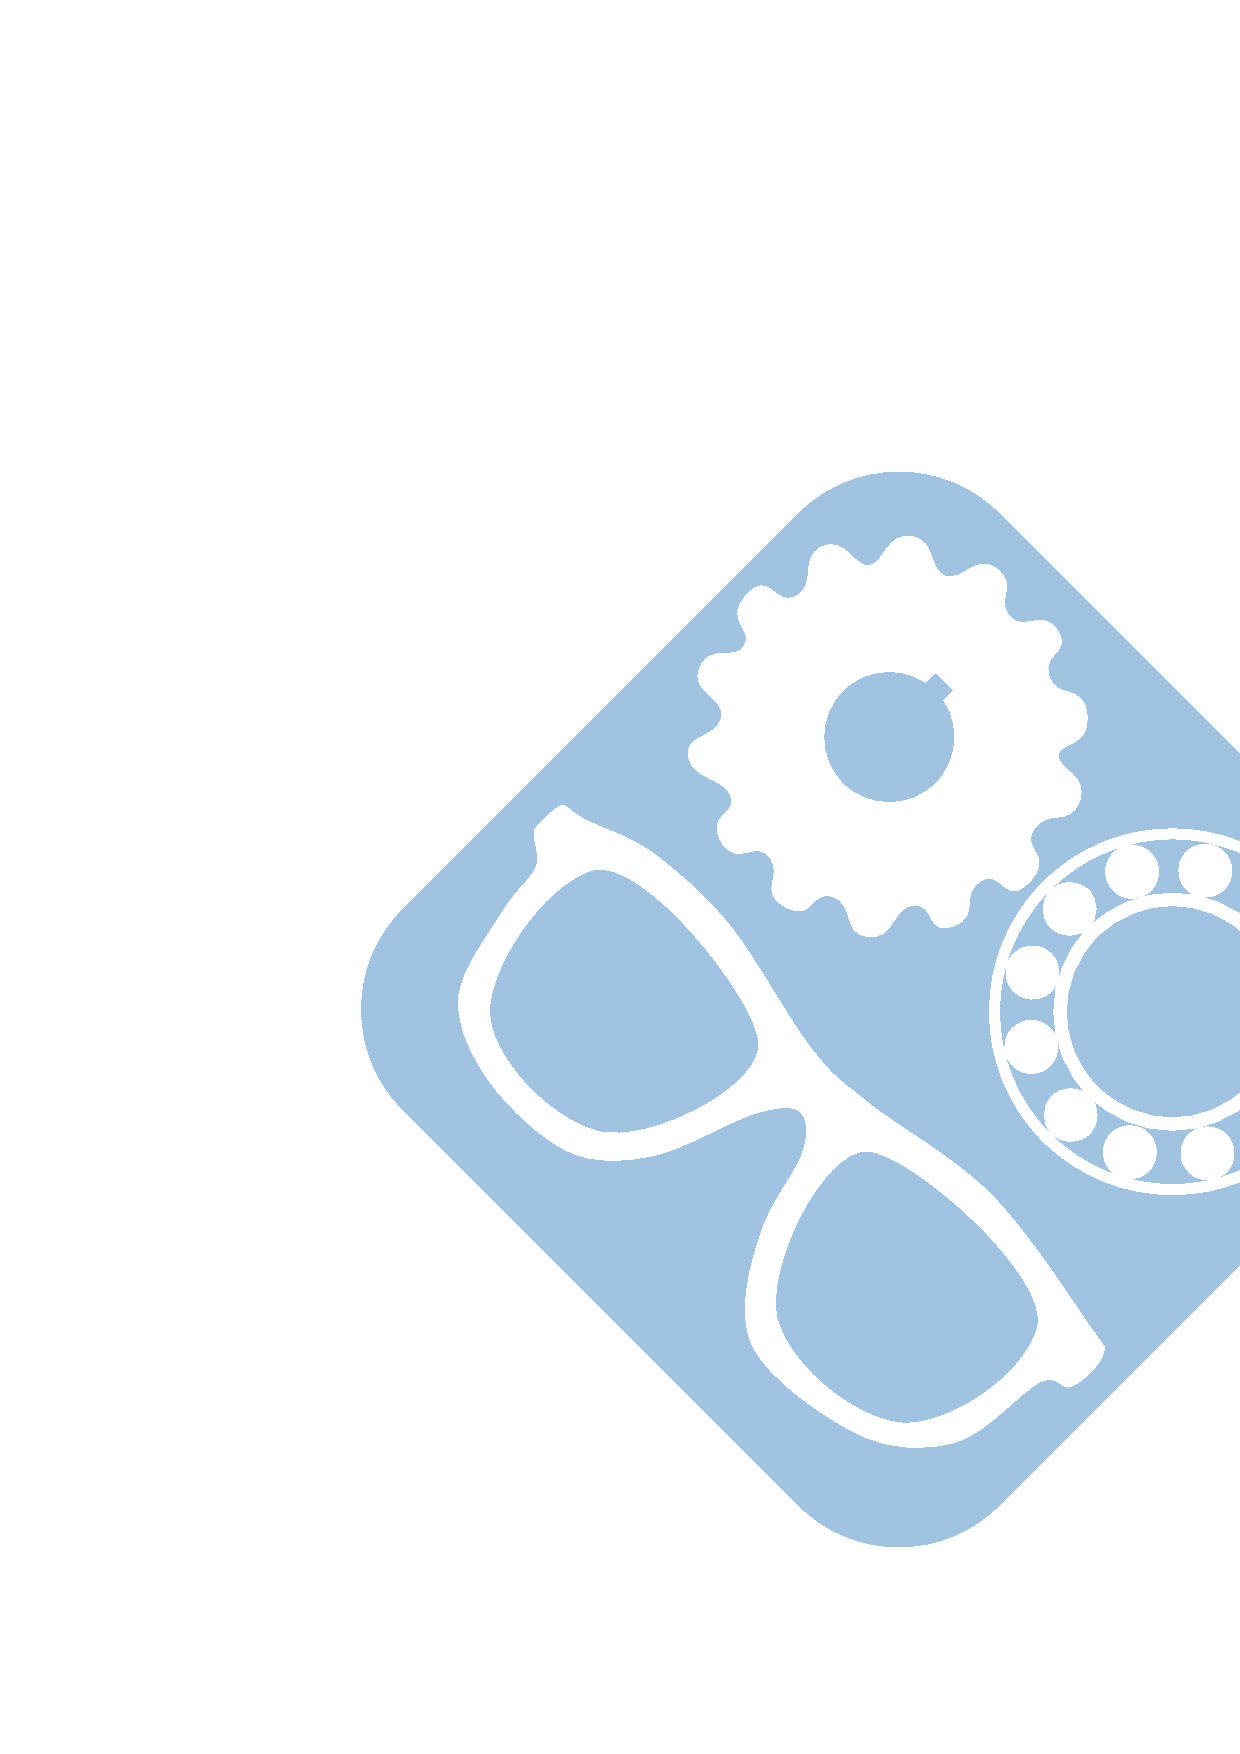
\includegraphics[width=\paperwidth,height=\paperheight,%
keepaspectratio]{../../img/fond3}%
\end{center}
\vfill
}}}

\newcommand{\BackgroundPicdeux}{%
\put(25,-30){%
\parbox[b][\paperheight]{\paperwidth}{%
\vfill
\begin{center}
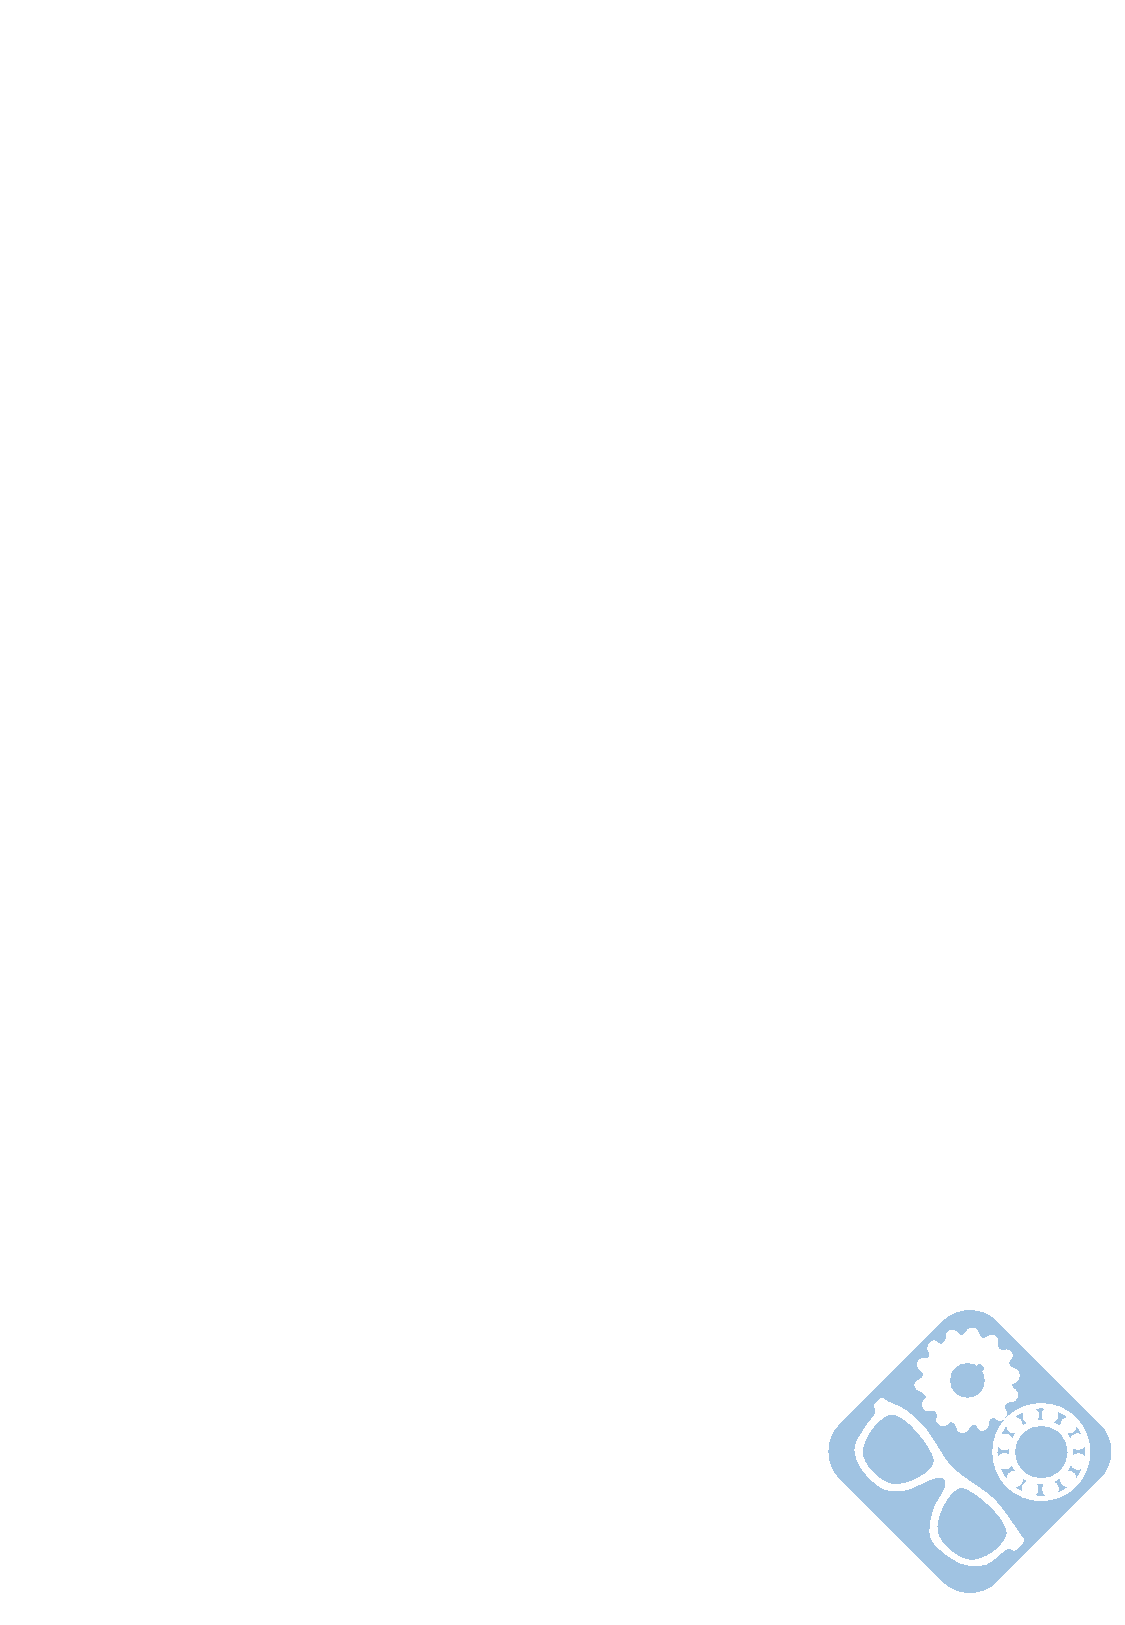
\includegraphics[width=\paperwidth,height=\paperheight,%
keepaspectratio]{../../img/fond4}%
\end{center}
\vfill
}}}

\begin{document}

\pagestyle{empty}

\vspace*{-3\baselineskip}

\AddToShipoutPicture*{\BackgroundPic}

\ifdef{\auteurdeux}{\begin{tabular}{>{\columncolor{gray!00}}m{.3\linewidth} m{.3\linewidth} >{\columncolor{gray!00}}m{.3\linewidth}}
Séquence : \sequence &  \multirow{3}{*}{\hspace{1cm}
\includegraphics[height=1.5cm]{../../img/logo}} &  \begin{flushright} \multirow{4}{*}{\hspace{1cm}
\includegraphics[height=4cm]{img/qrcode}}\end{flushright}\\
Document : \type\num \\
 \institute \\
 \auteurun\\
 \auteurdeux
\end{tabular}}{\begin{tabular}{>{\columncolor{gray!00}}m{.3\linewidth} m{.3\linewidth} >{\columncolor{gray!00}}m{.3\linewidth}}
Séquence : \sequence &  \multirow{3}{*}{\hspace{1cm}
\includegraphics[height=1.5cm]{../../img/logo}} &  \begin{flushright} \multirow{4}{*}{\hspace{1cm}
\includegraphics[height=4cm]{img/qrcode}}\end{flushright}\\
Document : \type\num \\
 \institute \\
 \auteurun
\end{tabular}}

\vspace{1cm}

\ifdef{\prive}{\begin{center}\colorbox{danger}{\Huge{Avec Correction}}\end{center}}{}

\begin{center}\huge{\nom}\end{center}

\vspace{2cm}

\ifdef{\imagedeux}{\begin{minipage}{0.49\linewidth}}{}
\begin{center}\includegraphics[height=5cm]{/home/renaud/Documents/Renaud/GitHub/django_education/systemes/\imageun}\end{center}
\ifdef{\imagedeux}{\end{minipage}\hfill
\begin{minipage}{0.49\linewidth}
\begin{center}\includegraphics[height=5cm]{/home/renaud/Documents/Renaud/GitHub/django_education/systemes/\imagedeux}\end{center}
\end{minipage}}{}

\vspace{5cm}


\begin{tabular}{p{.15\linewidth} >{\columncolor{white}}p{.8\linewidth}}
    \rowcolor{gray!20}
    Référence & S\sequence\ - \type\num \\
    Compétences & \competences \\
 	\rowcolor{gray!20}
    Description & \descrip \\
    Système & \systemes
  \end{tabular}

\newpage

\AddToShipoutPicture{\BackgroundPicdeux}

\pagestyle{normal}

\section{Définition du système}

\begin{minipage}{0.55\linewidth}
  Les fixations sont soumises aux variations de température, à l'humidité, à des efforts importants et à l'agression des skis des autres skieurs, notamment dans les files d'attente des remontées mécaniques.
  Les fixations sont des \og organes de sécurité \fg, elles sont des éléments essentiels de la sécurité du skieur. Leur rôle est de maintenir la chaussure sur le ski :
  \begin{itemize}
   \item Assez fermement pour ne pas décrocher au passage des bosses et des creux, tout en absorbant vibrations et chocs,
   \item Avec un déclenchement programmé pour protéger le genou en cas de chute.
  \end{itemize}
 \end{minipage}
 \hfill
  \begin{minipage}{0.4\linewidth}
   \centering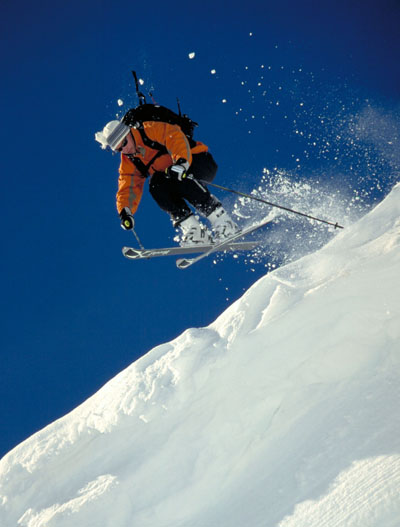
\includegraphics[width=0.7\linewidth]{img/skieur.jpg}
  \end{minipage}

\subsection{Définition du système : Principe de fonctionnement}

En cas de chute, la fixation doit se déclencher pour un couple défini par la norme ISO 11088 pour éviter une forte sollicitation du genou :
\begin{itemize}
 \item à la torsion,
 \item à la flexion.
\end{itemize}

Sur les figures suivantes, le mouvement de la chaussure sera représenté en blanc et celui de la talonnière (T) en vert, la butée est désignée par la lettre (B).

\textbf{En torsion droite ou gauche}

\begin{minipage}{0.4\linewidth}
   \centering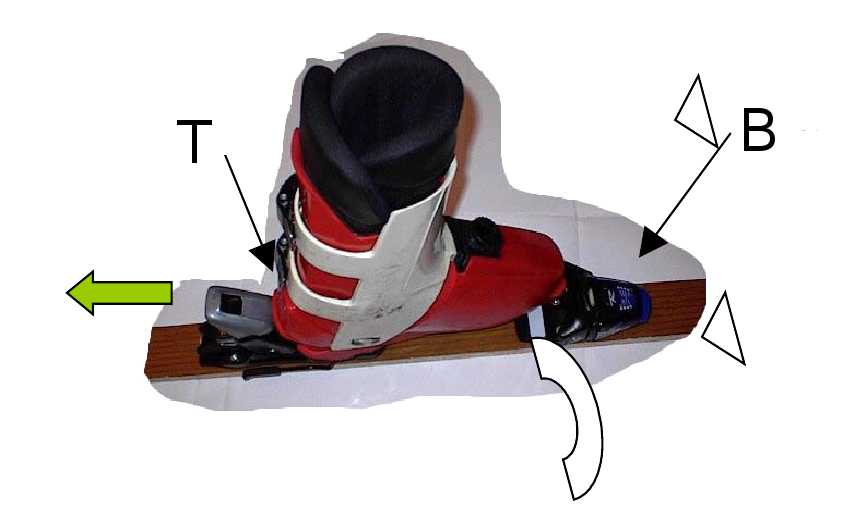
\includegraphics[width=0.9\linewidth]{img/torsion_droite.png}
 \end{minipage}
 \hfill
  \begin{minipage}{0.55\linewidth}
  La talonnière recule, le mors de butée s'écarte, la chaussure est libérée.
  \end{minipage}

\textbf{En chute avant}

\begin{minipage}{0.4\linewidth}
   \centering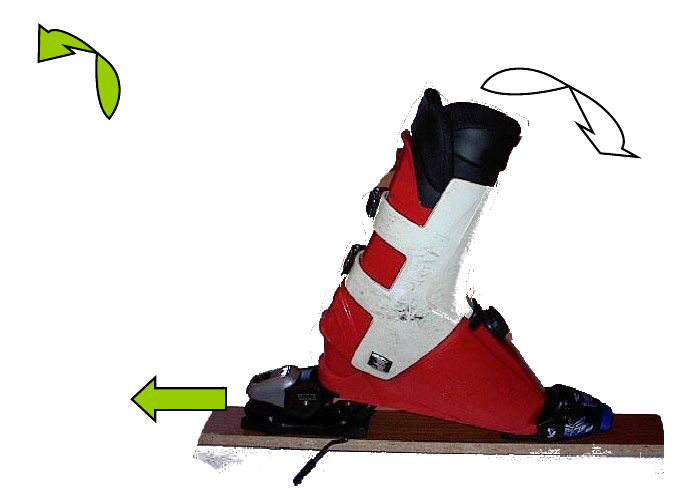
\includegraphics[width=0.9\linewidth]{img/Chute-avant.png}
 \end{minipage}
 \hfill
  \begin{minipage}{0.55\linewidth}
    La talonnière recule, l'agrippe-talon pivote, la chaussure est libérée.
  \end{minipage}

\textbf{Un maintient constant}

Au passage des creux et des bosses, les skis subissent une flexion importante alors que la semelle des chaussures est rigide (cote L constante). Pour éviter de se décrocher, la talonnière recule ou avance pour garder le contact avec la chaussure.

 \begin{minipage}{0.3\linewidth}
   \centering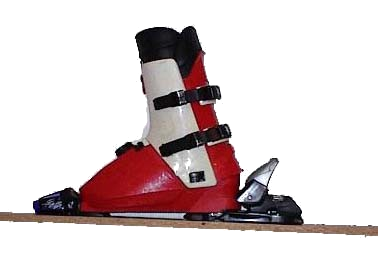
\includegraphics[width=0.8\linewidth]{img/normal.png}
 \end{minipage}
 \hfill
  \begin{minipage}{0.3\linewidth}
   \centering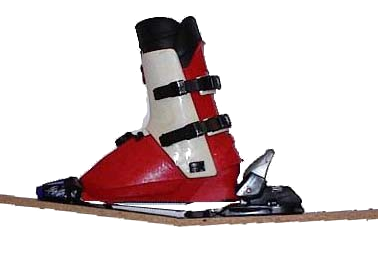
\includegraphics[width=0.8\linewidth]{img/reduc.png}
  \end{minipage}
 \hfill
  \begin{minipage}{0.3\linewidth}
   \centering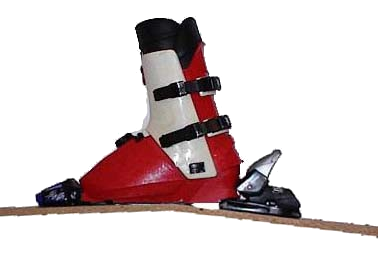
\includegraphics[width=0.8\linewidth]{img/augmen.png}
  \end{minipage}


\begin{center}
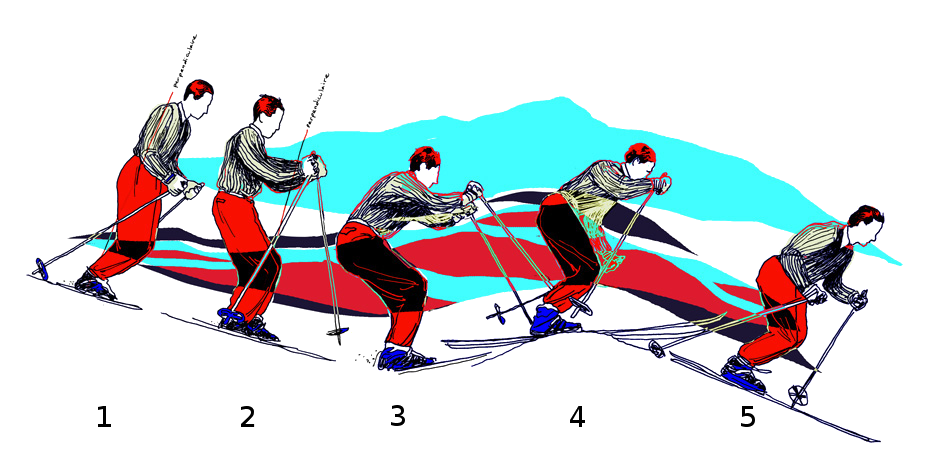
\includegraphics[width=0.8\linewidth]{img/passage_bosse.png}
\end{center}

\subsection{Etude de la talonnière}

La talonnière est l'organe de la fixation situé à l'arrière de la chaussure.

\begin{center}
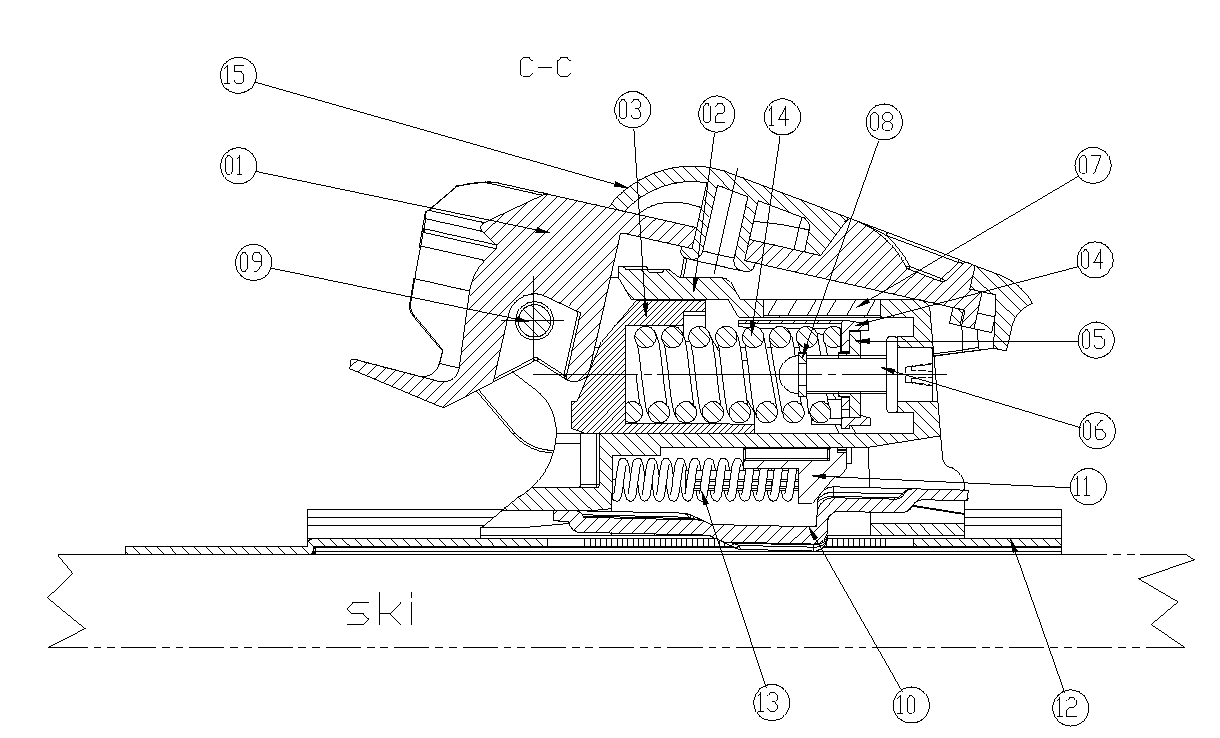
\includegraphics[width=0.7\linewidth]{img/talonniere.png}
\end{center}

 \begin{minipage}{0.3\linewidth}
   \centering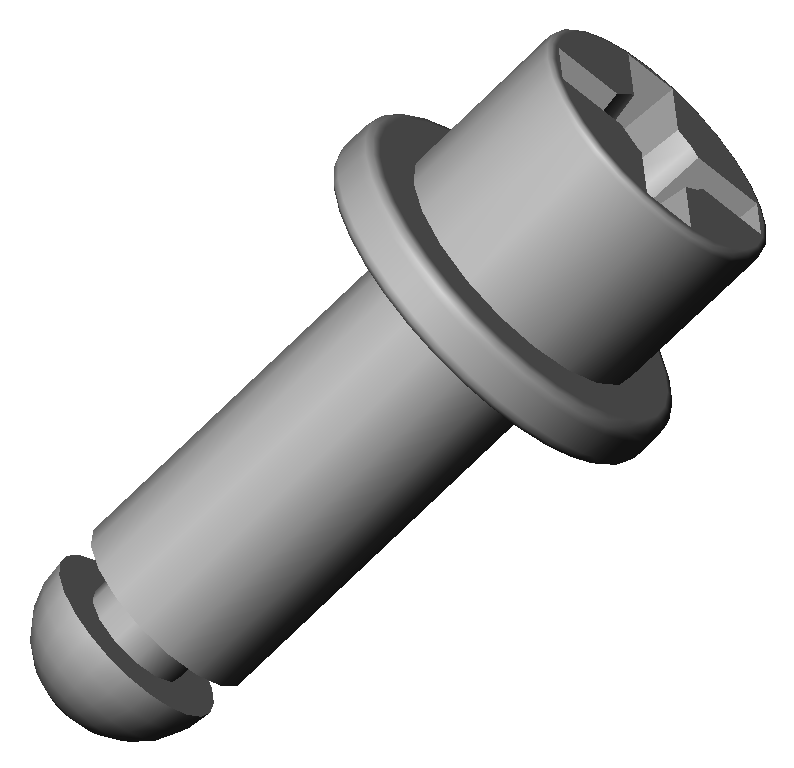
\includegraphics[height=4cm]{img/vis.png}
 \end{minipage}
 \hfill
  \begin{minipage}{0.3\linewidth}
  \centering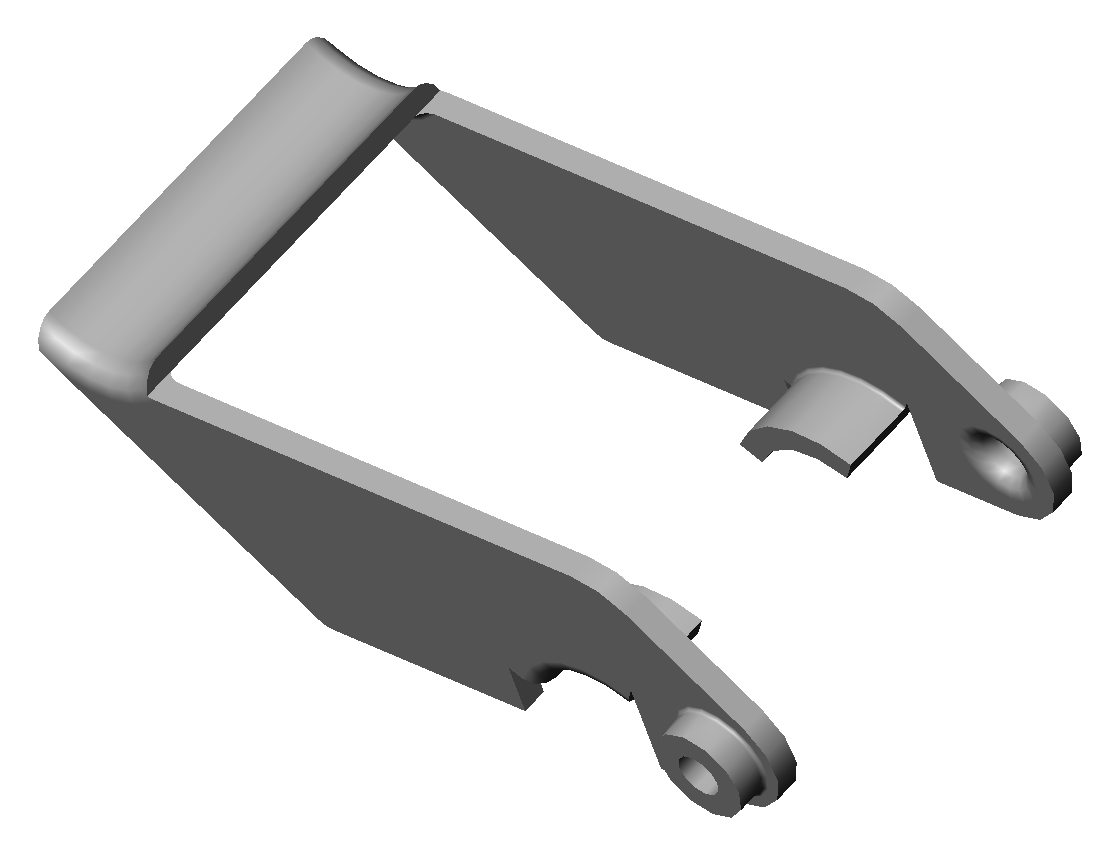
\includegraphics[height=5cm]{img/levier_reglage.png}
  \end{minipage}

\begin{center}
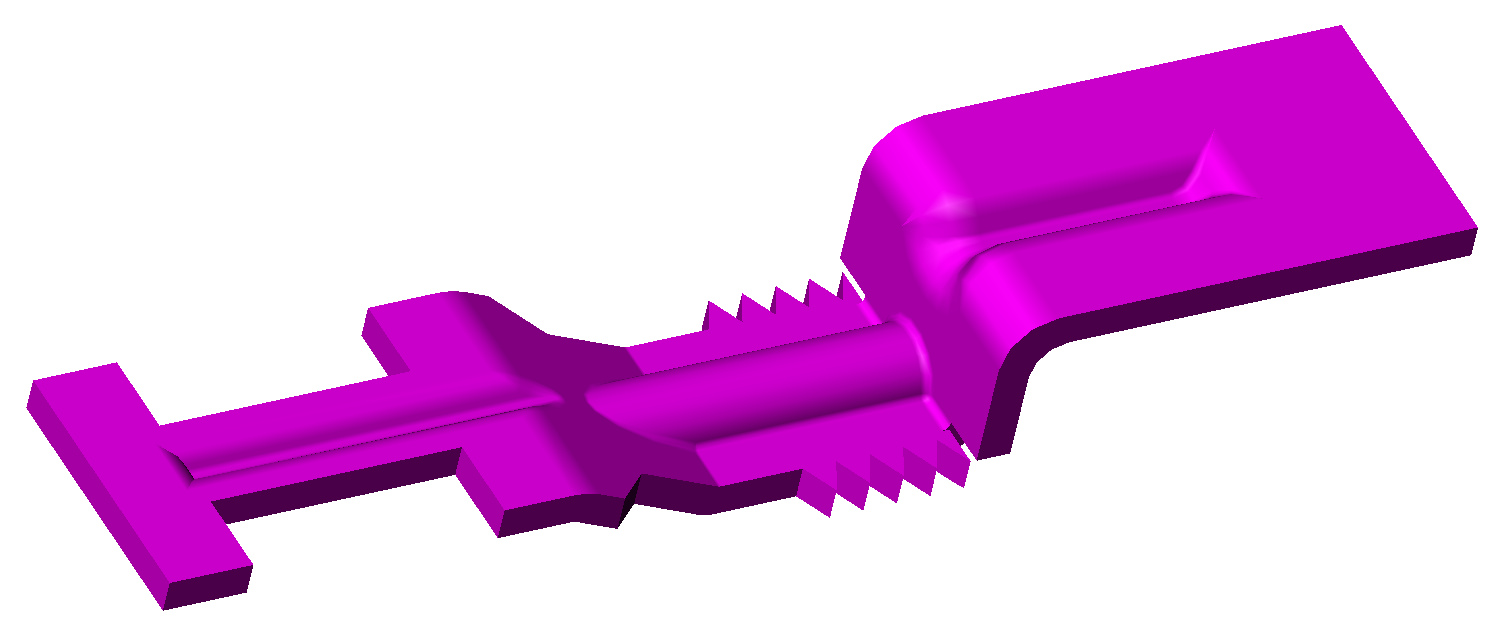
\includegraphics[width=0.8\linewidth]{img/barrette_reglage.png}
\end{center}

\section{Analyse fonctionnelle du système}

\paragraph{Question 1:}

Réaliser un diagramme des exigences du système.

\section{Analyse cinématique}

\paragraph{Question 2:}

A partir de la vue en coupe de la talonnière, déterminer les sous-ensembles cinématiquement liés.

\begin{table}[!h]
 \centering\begin{tabular}{|m{5cm}|m{8cm}|}
 \hline
 S1 & 1, \\
 \hline
 S2 & 2, \\
 \hline
 S3 & 3, \\
 \hline
 S4 & 12, \\
 \hline
 Éléments déformables & \\
 \hline
 \end{tabular}
\end{table}

\paragraph{Question 3:}

Établir le graphe des liaisons du système.

\vspace{5cm}

\paragraph{Question 4:}

Établir le schéma cinématique du système.

\vspace{5cm}

\section{Analyse de la fabrication}

On donne les représentations de certaines pièces de la fixation. Leurs bruts ont été mis en forme par forgeage. Ces pièces sont disponibles sur le modèle SolidWorks du système.

\subsection{Vis de réglage de dureté}

\textit{Les vidéos de présentation des étapes de la fabrication des vis peut vous aider à répondre à cette question.}

 \begin{minipage}{0.3\linewidth}
    \centering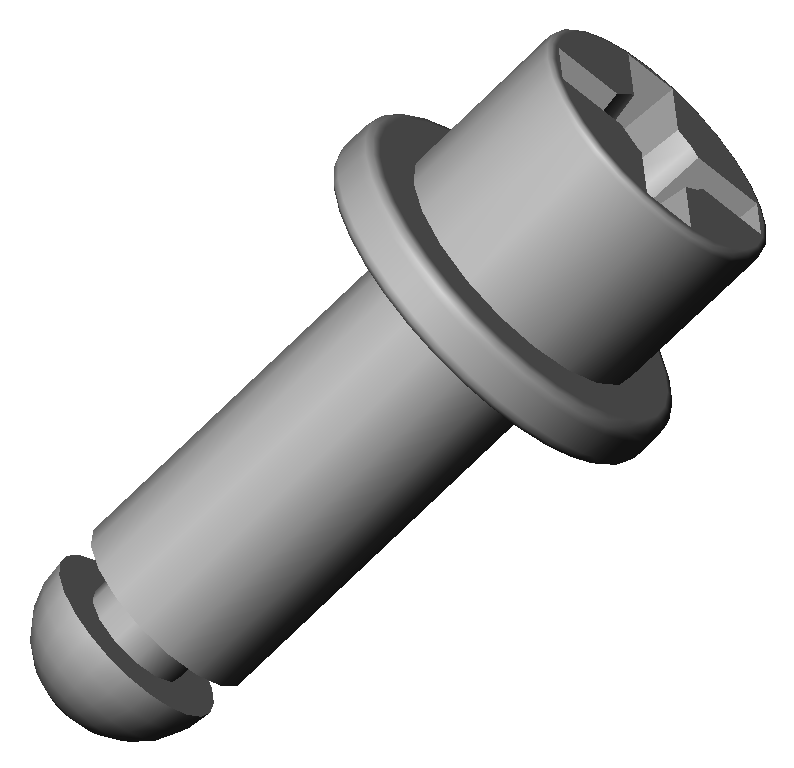
\includegraphics[width=1\linewidth]{img/vis.png}
 \end{minipage}
 \hfill
 \begin{minipage}{0.65\linewidth}
 \paragraph{Question 5:} Quel procédé de fabrication a été utilisé pour mettre en forme cette pièce?
 
 \end{minipage}


\paragraph{Question 6:} Dessiner à main levée l'évolution de la géométrie de la pièce d'un cylindre plein jusqu'à la géométrie finale.

\vspace{5cm}

\subsection{Levier de réglage}


 \begin{minipage}{0.3\linewidth}
 \centering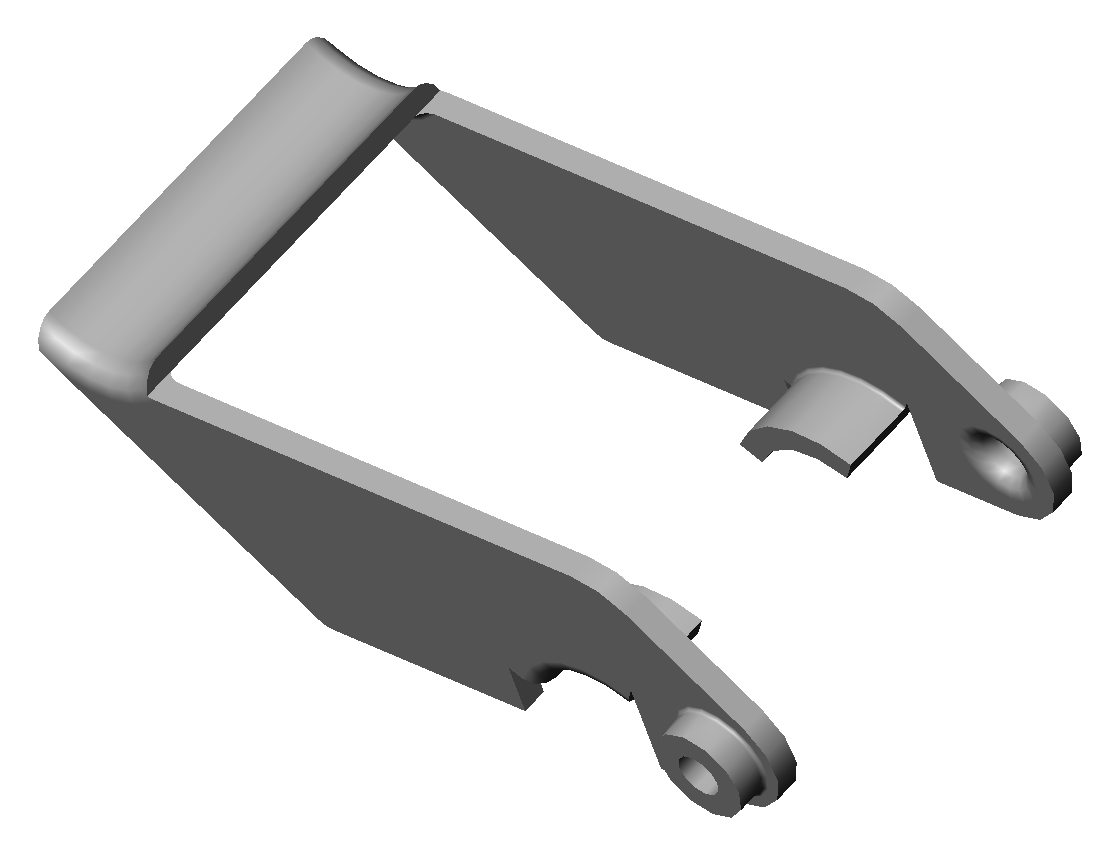
\includegraphics[width=1\linewidth]{img/levier_reglage.png}
 \end{minipage}
 \hfill
 \begin{minipage}{0.65\linewidth}
 \paragraph{Question 7:} Quel procédé de fabrication a été utilisé pour mettre en forme cette pièce?

 \end{minipage}


\paragraph{Question 8:} Dessiner à main levée l'évolution de la géométrie de la pièce d'une tôle jusqu'à la géométrie finale.

\vspace{5cm}

\subsection{Barrette de réglage}


 \begin{minipage}{0.3\linewidth}
 \centering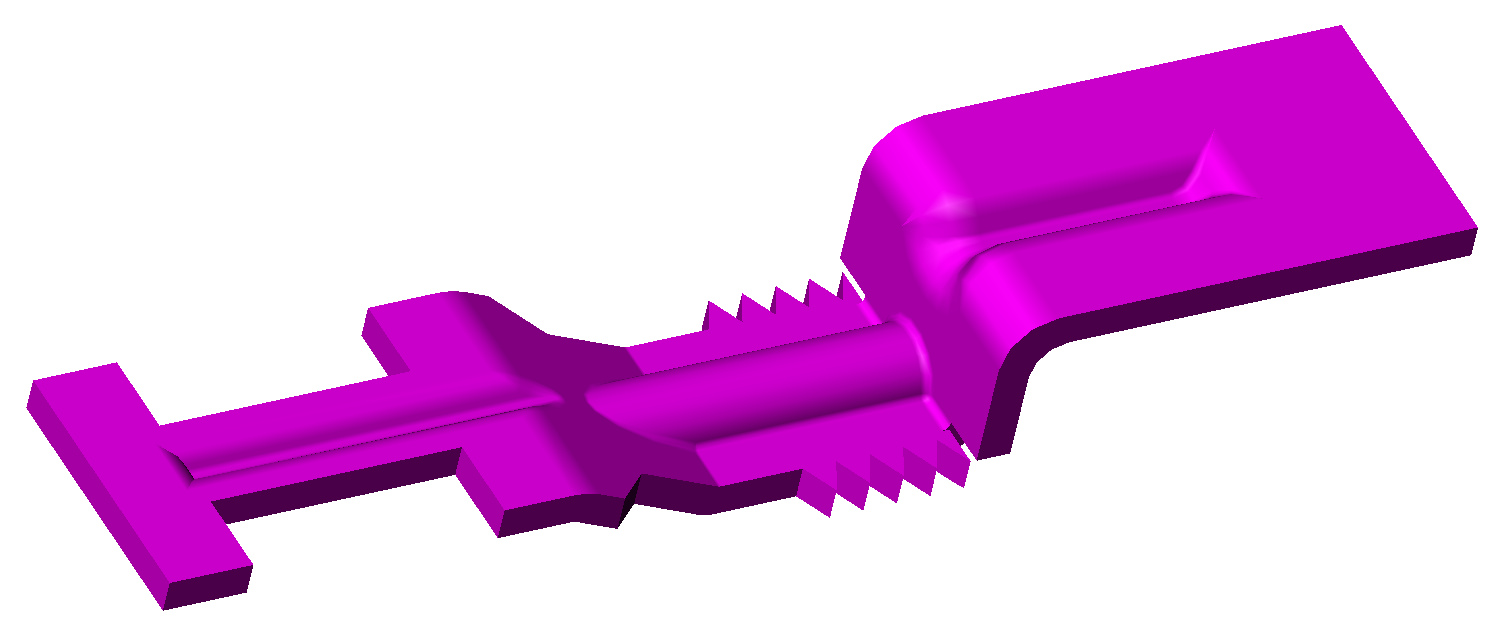
\includegraphics[width=1\linewidth]{img/barrette_reglage.png}
 \end{minipage}
 \hfill
 \begin{minipage}{0.65\linewidth}
 \paragraph{Question 9:} Quel procédé de fabrication a été utilisé pour mettre en forme cette pièce?

 \end{minipage}

\paragraph{Question 10:} Dessiner à main levée l'évolution de la géométrie de la pièce d'une tôle jusqu'à la géométrie finale.

\vspace{5cm}

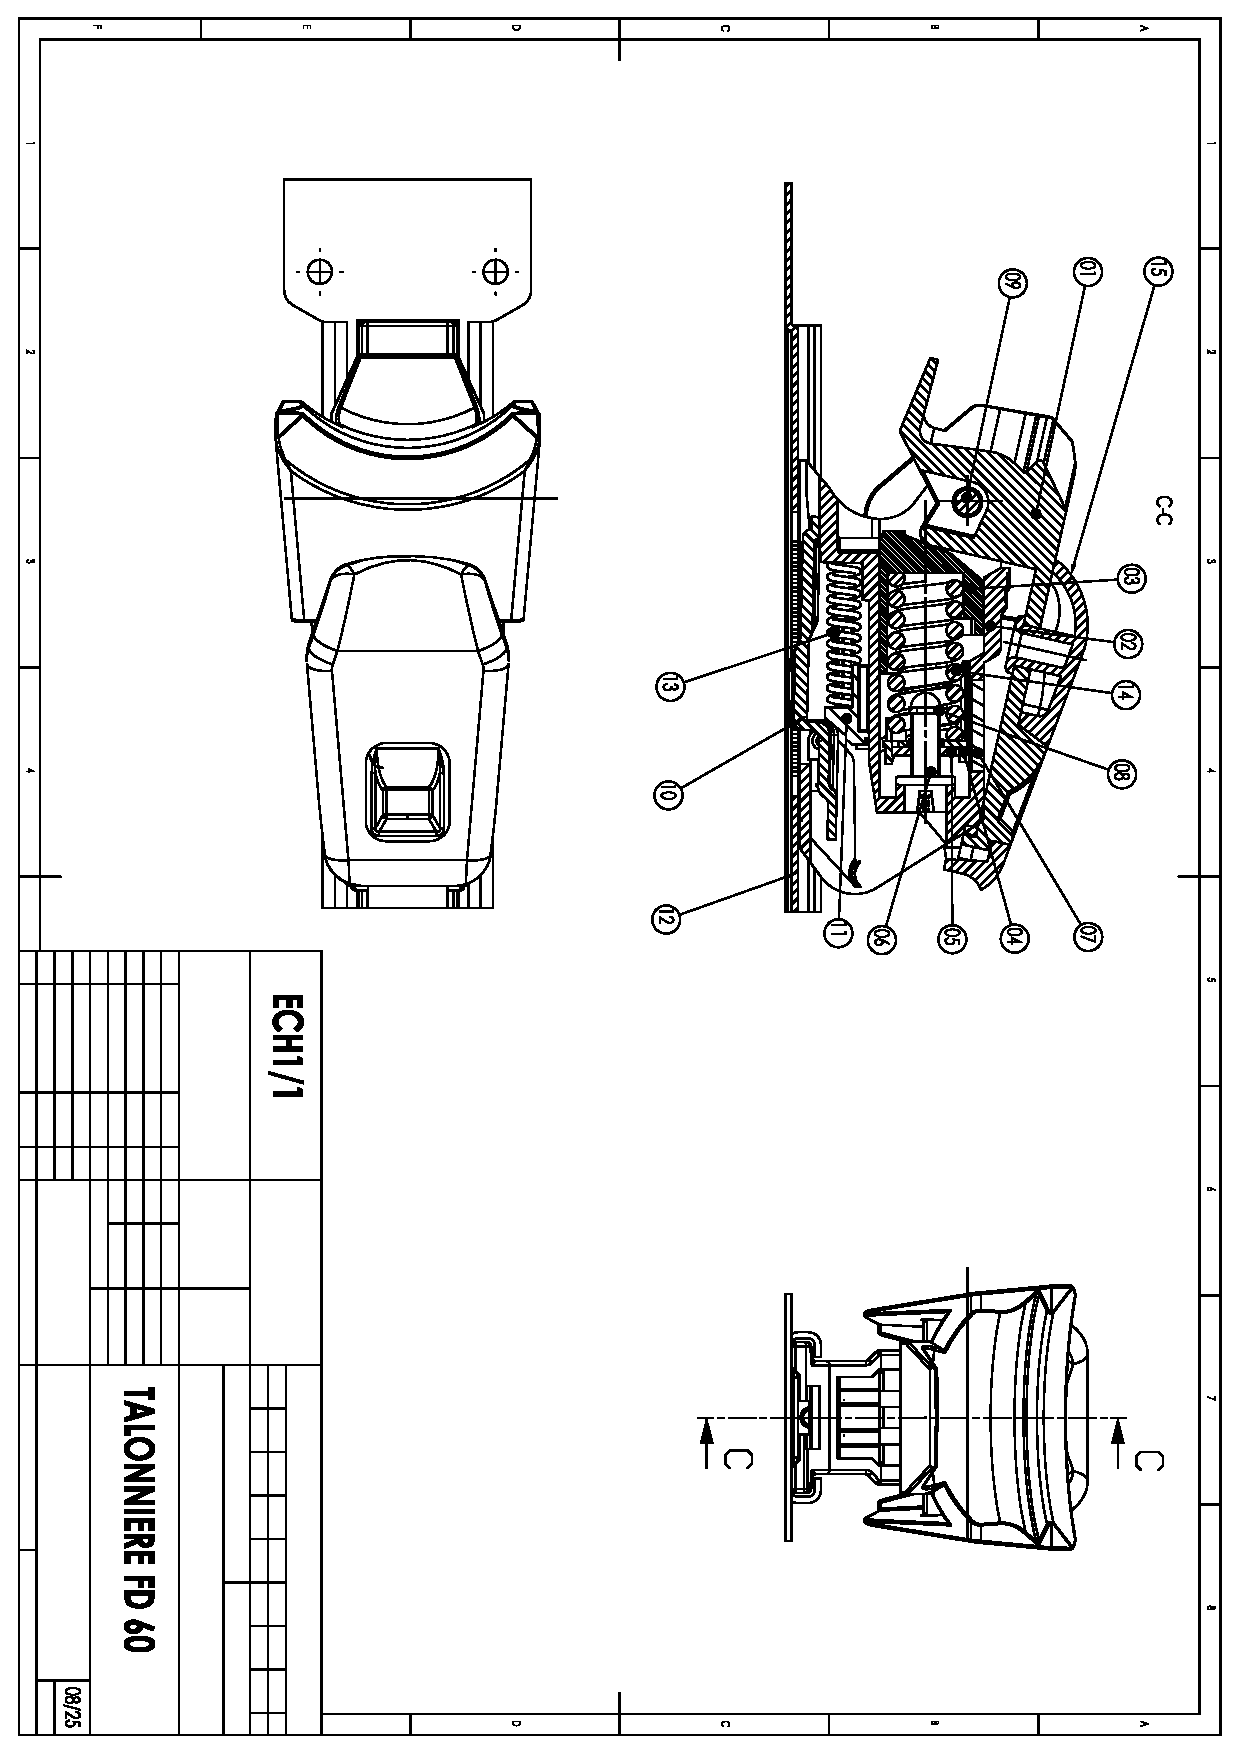
\includepdf[pages=1-5]{img/Plans.pdf}

\end{document}
